\documentclass[12 pt, a4paper, toc=graduated, oneside]{article}
\usepackage{amsmath, amssymb,amsfonts, amsthm, mathtools}
\usepackage[utf8]{inputenc}
\usepackage[inline]{enumitem}
\usepackage[colorlinks=true]{hyperref}
\usepackage{geometry}
 \geometry{
 a4paper,
 total={170mm,257mm},
 left=20mm,
 top=20mm,
 }

\setlength\parindent{0 pt}

\theoremstyle{definition}
\newtheorem{defn}{Definition}
\newtheorem{theorem}{Theorem}
\newtheorem{lem}{Lemma}
\newtheorem{cor}{Corollary}

\title{MA 419: Basic Algebra}
\author{Aryaman Maithani}
\date{Autumn 2019}

\usepackage{tikz-cd}
\usepackage{tikz}

\usepackage{xcolor}
\definecolor{mybgcolor}{RGB}{50, 50, 50} %46, 51, 63

\usepackage{pagecolor}
%\pagecolor{mybgcolor}
%\color{white}

\newcommand{\pset}{\raisebox{.15\baselineskip}{{\Large\ensuremath{\wp}}}}
\newcommand{\lcm}{\operatorname{lcm}}
\newcommand{\sign}{\operatorname{sign}}
\newcommand{\im}{\operatorname{im}}
\newcommand{\Aut}{\operatorname{Aut}}
\newcommand{\Syl}{\operatorname{Syl}}
\newcommand{\ord}{\operatorname{ord}}

\begin{document}
\maketitle
\tableofcontents
%\addtocontents{toc}{~\hfill\textbf{Page}\par}
\newpage
%
\section{Groups}
Let $G$ be a set with an associative law of composition $\cdot.$ $(G, \cdot)$ is called a group if it has an identity element and every element of $G$ is invertible.\\
That is,
\begin{enumerate}[nosep]
	\item $\exists e \in G: \forall g \in G: e\cdot g = g = g\cdot e.$
	\item $\forall g \in G: \exists g' \in G: g\cdot g' = e = g'\cdot g.$
\end{enumerate}

We often shorten $a\cdot b$ and write $ab$ instead.\\
$e$ is often denoted by $1.$\\~\\
\textbf{Example}:\\
$S_3 = \langle x, y | x^3 = 1, y^2 = 1, yx = x^2y\rangle$
\section{Subgroup}
Let $(G, \cdot)$ be a group and $H \subset G.$\\
$H$ is a subgroup of $H$ if:
\begin{enumerate}[nosep] 
	\item $\cdot|_H$ is a binary operation on $H.$ (Closure)
	\item $(H, \cdot|_H)$ is a group.\\
\end{enumerate}
Notation: $H \le G.$
\subsection{Subgroups of \texorpdfstring{$\mathbb{Z}$}{Z}}
\begin{enumerate}
	\item Given $n \in \mathbb{Z},$ define $n\mathbb{Z} := \{nm | m \in \mathbb{Z}\}.$
	\item Given $a, b \in \mathbb{Z},$ define $a\mathbb{Z} + b\mathbb{Z} = \{an + bm | n, m \in \mathbb{Z}\}.$ 
	\item If $H \le \mathbb{Z},$ then $H = \{0\}$ or $H = n\mathbb{Z}$ where $n$ is the smallest positive element of $H.$
	\item $a\mathbb{Z} + b\mathbb{Z}$ is the smallest subgroup of $\mathbb{Z}$ containing $a$ and $b.$
	\item If $(a, b) \neq (0, 0),$ then the smallest positive element of $a\mathbb{Z} + b\mathbb{Z}$ is defined to be $\gcd(a, b).$
	\item If $\lcm(a, b) = l,$ then $\langle l \rangle$ is the largest subgroup of $\langle a\rangle \cap \langle b\rangle.$
\end{enumerate}
\section{Order and Cyclic groups}
Let $G$ be a group and $x \in G.$\\
\begin{defn}
	$\langle x\rangle$ is the smallest subgroup of $G$ containing $x.$\\
	$\langle x\rangle = \{\cdots, x^{-2}, x^{-1}, 1, x, x^2, \cdots\}.$\\
\end{defn}
\begin{defn}
	Order of an element $x$ of $G$ is denoted by $o(x)$ and is defined as $o(x) := |\langle x\rangle|.$\\~\\
	$G$ is said to be cyclic if there exists $x \in G$ such that $\langle x\rangle = G.$
\end{defn}

\section{Sign of permutations}
Given $\sigma \in S_n,$ $\sigma$ has a matrix associated to it. Denote it by $[\sigma].$\\
$\operatorname{sign}(\sigma) := \det([\sigma]).$\\
The sign of any transposition is $-1.$\\
As any element of $S_n$ can be written as a product of transpositions, the sign is always $\pm 1.$\\
Permutations with sign $1$ are called even permutations and the rest are called odd permutations.\\
The set of even permutations is denoted by $A_n.$

\section{Homomorphisms}
\begin{defn}
	Let $G$ and $G'$ be groups.\\
	A map $\alpha:G\to G'$ is said to be a group homomorphism if:
	\[\alpha(g_1g_2) = \alpha(g_1)\alpha(g_2) \quad \forall g_1, g_2 \in G.\]
\end{defn}
(High abuse of notation has been done.)

\begin{defn}
	Let $\alpha : G \to G'$ be a homomorphism.\\
	$\ker \alpha := \{g \in G | \alpha(g) = 1\} = \alpha^{-1}(1).$\\
	$\im \alpha := \{\alpha(g) | g \in G\}.$
\end{defn}
Fact: $\ker \alpha \le G$ and $\im \alpha \le G'.$\\
$\alpha$ is 1-1 $\iff \ker \alpha = \{1\}.$ 

\section{Conjugates, normal subgroup, normaliser, center}
\begin{defn}
	$G \to$ group. Let $a, g \in G.$ Then the element is $gag^{-1}$ of $G$ is said to be the \textbf{conjugate} of $a$ by $g.$ 
\end{defn}
\begin{defn}
	Let $H \le G.$ $H$ is called a \textbf{normal subgroup} of $G$ if
	\[\forall h \in H, \forall g \in G: ghg^{-1} \in H.\]
	Notation: $H \trianglelefteq G.$
\end{defn}
Fact: If $K$ is the kernel of $\varphi:G\to G',$ then $K \trianglelefteq G.$\\
Remark: Suppose $G$ is generated by $g_1, g_2, \cdots, g_n.$ Let $H \le G.$ Then
\[H \trianglelefteq G \iff \forall i \in [n], \forall h \in H: g_ihg_i^{-1} \in H\]
\begin{defn}
	Let $g\in G.$ Define $C_g:G\to G$ as $x \mapsto gxg^{-1}$ under $C_g.$
\end{defn}
$C_g$ is a homomorphism for all $g \in G.$ In fact, it is an isomorphism.
\begin{defn}
	Let $H \le G.$\\
	The \textbf{normaliser} of $H$ in $G$ is defined as -
	\[N_G(H) := \{g \in G \mid gHg^{-1} = H\}.\]
\end{defn}
$N_G(H) \le G.$
\begin{defn}
	The \textbf{center} of a group $G$ is defined -
	\[Z(G) := \{g \in G \mid \forall x \in G: gx = xg\}.\]
\end{defn}
$Z(G) \trianglelefteq G.$

\section{Isomorphisms}
\begin{defn}
	$\varphi : G \to G' \longleftarrow$ homomorphism\\
	If $\varphi$ is bijective, then we say that $\varphi$ is an isomorphism.
\end{defn}
\begin{defn}
	Let $G$ and $G'$ be groups. If there exists $\varphi:G \to G'$ such that $\varphi$ is an isomorphism, then we say that $G$ and $G'$ are isomorphic.
\end{defn}
Facts:
\begin{enumerate}[nosep] 
	\item $\varphi$ is an isomorphism $\iff$ $\ker \varphi = (1)$ and $\varphi$ is onto.
	\item If $\varphi:G\to G'$ is a 1-1 homomorphism, then $\bar{\varphi}:G\to \im G \;(\le G')$ is an isomorphism.
	\item Let $\varphi:G \to G'$ be an isomorphism. Let $\varphi^{-1}$ be the set theoretic inverse of $\varphi.$ Then, $\varphi^{-1}$ is a homomorphism and hence, an isomorphism.
\end{enumerate}
Given any set of groups, the relation ``is isomorphic to'' is an equivalence relation.
\begin{defn}
	$\operatorname{Aut} G := \{\varphi : G \to G \mid \varphi \text{ is a bijection}\}.$\\
	Elements of the above set are called automorphisms of $G.$
\end{defn}
$\operatorname{Aut} G$ is a group under composition.\\
\textbf{Example:}
\begin{enumerate}[nosep] 
	\item Let $G$ be a group. Fix $g \in G.$ Define $\varphi_G:G \to G$ as $x \mapsto gxg^{-1}.$\\
	This is an automorphism.
	\item $\varphi_g = \text{id} \iff \varphi_g(x) = x \; \forall x \in G \iff g \in Z(G).$
\end{enumerate}
%
\section{Cosets}
\begin{defn}
	Let $G \longleftarrow$ group and $H \le G.$ For $a \in G,$ $aH := \{ah : h \in H\}.$ This is said to be a left coset of $H$ by $a.$
\end{defn}
\begin{defn}
	$G \longleftarrow$ group. $H \le G.$ Define $g \sim g'$ if $g = g'h$ for some $h \in H.$
\end{defn}
This $\sim$ is an equivalence relation.\\
Thus, $G$ is the disjoint union of left cosets of $H$ in $G.$\\
Also, given $g,\; g'\in G,$ it either the case that $gH = g'H$ or that $gH \cap g'H = \emptyset.$\\
Facts:
\begin{enumerate}[nosep] 
	\item $gH \le G \iff g \in H.$
	\item Fix $g, g' \in G.$ Then, we can have a map $\varphi:gH \to g'H$ such that $gh \mapsto g'h.$ (Check that this is well-defined.)\\
	Then, $\varphi$ is a bijection. $\implies |gH| = |g'H|.$
\end{enumerate}
\begin{defn}
	$[G:H] := $ index of $H$ in $G$\\
	= Number of distinct left cosets of $H$ in $G.$ \hfill (may be $\infty$)\\
	= Number of equivalence classes
\end{defn}
By the last fact given above, we have it that $G$ is the disjoint union of $[G:H]$ many left cosets of $H.$\\
Therefore, $|G| = [G:H] |H|.$ \hfill (For finite)
\begin{theorem}
	$G \longleftarrow$ finite group and $H \le G.$ Then, $|H| \mid |G|.$
\end{theorem}
\begin{theorem}
	$|G| = p \longleftarrow$ prime. Then $G$ is cyclic and has $p-1$ generators.
\end{theorem}
If $\varphi:G \to G'$ is a homomorphism, $\varphi:G \to \im \varphi$ is onto and $\im \varphi \le G'.$\\
If $g' \in \im \varphi,$ then there exists $g \in G$ such that $g' = \varphi(g).$ Let $K = \ker \varphi.$\\
$\varphi^{-1}(g') = \{x \in G : \varphi(x) = g'.\}$ Then, $\varphi^{-1}(g') = gK.$\\
Also, $\{\text{cosets of }K\text{ in }G\} \cong \im \varphi$ (set isomorphism, i.e., bijection).\\
$gK \mapsto \varphi(g)$ is the map.\\
$\therefore |\im \varphi| = [G:K].$\\
$|G| = [G:K]|K| \implies |G| = |\im \varphi|\cdot|K|.$ \\
For finite $G$ and $G',$ we have it that $|\im\varphi|$ divides $|G|$ and $|\im\varphi|$ divides $G'.$\\
Ex.: The above can use to shown that $|A_n| = n!/2$ for $n \ge 2.$\\
(Consider the (onto) homomorphism $\sign:S_n \to \{-1, 1\}.$)

\section{A lemma on normal subgroups}
\begin{lem}
	$G \longleftarrow$ group. $H \le G.$ TFAE:
	\begin{enumerate}[nosep] 
		\item $H \trianglelefteq G.$ That is, $\forall g \in G, \forall h \in H : ghg^{-1} \in H.$
		\item $gHg^{-1} = H \forall g \in G.$
		\item Any left coset of $G$ is also a right coset.
	\end{enumerate}
\end{lem}

\section{Correspondence Theorem}
Let $\varphi:G \to G'$ be a group homomorphism.
\begin{enumerate}[nosep] 
	\item If $H \le G,$ then $\varphi(H) \le G'.$
	\item Let $H \trianglelefteq G,$ it is not necessary that $\varphi(H) \trianglelefteq G'.$
	\item Assume $\varphi$ is surjective. Now, if $H \trianglelefteq G,$ then $\varphi(H) \trianglelefteq G'.$
	\item If $H' \trianglelefteq G',$ then $\varphi^{-1}(H') \trianglelefteq G.$ \hfill (No assumption of surjectivity.)
\end{enumerate}
\begin{theorem}
	Assume $\varphi : G \to G'$ is a surjective homomorphism.\\
	Then, $\Omega_1 = \{\text{All subgroups of } G \text{ containing } \ker \varphi\} \cong \{\text{All subgroups of }G'\} = \Omega_2.$
\end{theorem}
Consequence:\\
Consider $\det:GL_2(\mathbb{R}) \to \mathbb{R}^\times.$ This is a surjective map. Moreover, $\mathbb{R}^\times$ is abelian.\\
Thus, the set of subgroups of $GL_2(\mathbb{R})$ containing $SL_2(\mathbb{R})$ consists of abelian subgroups. Moreover, it is in bijection with the set of subgroups of $\mathbb{R}^\times.$\\
$\det^{-1}(\{\pm1\}) = SL_2(\mathbb{R}) \cup \{\det -1 \text{ matrices}\}.$

\section{Product of Groups}
\begin{defn}
	Let $G$ and $G'$ be groups.\\
	Then, the product $G \times G'$ is a group under component wise operation.
\end{defn}
That is, for $(g_1, g_1')$ and $(g_2, g_2')$ belonging to $G \times G',$ $(g_1, g_1)\cdot(g_2, g_2') = (g_1\cdot g_2, g_1' \cdot g_2').$\\
(Where the $\cdot$ has different meanings depending on the elements.)\\~\\
%
Now, we want to answer the following question - \\
Given a group $G,$ when can we say that there exist groups $G_1$ and $G_2$ such that $G \cong G_1 \times G_2$ where $G_1$ and $G_2$ are non-trivial.\\
Consider the following maps:

\begin{center}

\begin{tikzcd}
G_1 \arrow[rrd, "i_1"]  &  &                                          &  & G_1 \\
                        &  & G \arrow[rru, "p_1"] \arrow[rrd, "p_2"'] &  &     \\
G_2 \arrow[rru, "i_2"'] &  &                                          &  & G_2
\end{tikzcd}
\end{center}

$i_1(g_1) = (g_1, 1).$ $i_1$ is an injective group homomorphism.\\
Thus, $G_1 \cong \im i_1 = G_1 \times \{1\}.$\\
Similarly, $G_2 \cong \im i_1 = \{1\} \times G_2.$\\
Both the latter groups are subgroups of $G.$\\
Thus, a necessary condition is - $G$ must contain subgroups that are isomorphic to $G_1$ and $G_2.$\\
Also, let $p_1$	be defined as $p_1(g_1, g_2) = g_1.$ Then, $\ker p_1 = \{1\} \times G_2 \longleftarrow$ normal subgroup of $G.$\\
Similar observation can be made for $p_2.$\\
Thus, if $G \cong G_1 \times G_2,$ then $G$ contains normal subgroups $H_1$ and $H_2$ which are isomorphic to $G_1$ and $G_2.$ In fact, the following can be observed:\\
If $G \cong G_1 \times G_2,$ then there exists normal subgroups $H_1$ and $H_2$ of $G$ such that:
\begin{enumerate}[nosep] 
	\item $H_1 \cong G_1$ and $H_2 \cong G_2.$
	\item $H_1 \cap H_2 = (1).$
	\item $H_1 H_2 = G.$
\end{enumerate}
Where $H_1H_2 := \{h_1h_2 \in G : h_1 \in H, \; h_2 \in H\}.$\\
\textbf{Exercises:}
\begin{enumerate}[nosep] 
	\item $HK \le G$ if ($H\trianglelefteq G$ or $K \trianglelefteq G$).
	\item $HK \trianglelefteq G$ if ($H\trianglelefteq G$ and $K \trianglelefteq G$)
	\item $HK \le G$ iff $HK = KH.$
\end{enumerate}
Let $H, K \le G$ and $\varphi:H\times K \to G$ be defined as $(h, k) \mapsto hk.$\\
Then, $\im \varphi = HK \subset G.$\\
Let us see when $\varphi$ is a homomorphism.\\
We need $\varphi(h, k)\varphi(h', k') = \varphi(hh', kk')$\\
$\iff hkh'k' = hh'kk' \iff kh' = h'k.$\\
That is, elements of $K$ and $H$ commute.\\
Then, we have it that $HK = KH$ and thus, $HK \le G.$\\
(Note that $HK = KH$ does not imply that the elements of $H$ and $K$ individually commute. The latter is stronger and that is what implies homomorphism.)\\~\\
If we want $\varphi$ to be an isomorphism, we need $\im \varphi = HK = G.$\\
Also, we need $\varphi$ to be 1-1. Thus, $\ker \varphi = (1) = \{(1, 1)\}.$\\
If $(h, k) \in \ker \varphi,$ then we have it that $hk = 1$ or $h = k^{-1}.$ As $H$ and $K$ are both subgroups, this tells us that $h, k \in H \cap K.$ For the sake of isomorphism, we want $1$ to be the only element in $H \cap K.$ \\
Thus, we arrive at the conclusion that $H \cap K = \{(1, 1)\}.$\\~\\
Explicitly stating our results:\\
There exist $H, K \le G$ such that $\varphi:H\times K \to G$ given by $(h, k) \mapsto hk$ is an isomorphism iff
\begin{enumerate}[nosep] 
 	\item $hk = kh \quad \forall h \in H,\; k\in K,$
 	\item $H \cap K = (1),$ and
 	\item $HK = G.$
\end{enumerate} 
The first and third conditions let us conclude that $H \trianglelefteq G$ and $K \trianglelefteq G.$\\~\\
%
\textbf{Example:}\\
Let $G = GL_2(\mathbb{R})^+ := \{M \in GL_2(\mathbb{R}) : \det M > 0\}.$\\
Let $H = SL_2(\mathbb{R})$ and $K = \left\{\begin{pmatrix}
a & 0\\
0 & a\end{pmatrix} : a \in \mathbb{R}_{> 0} \right\}.$\\
Then, by above theorem $G \cong H \times K.$ (Can be verified that $H$ and $K$ satisfy the three criteria.)\\
Moreover, it can be seen that $K$ is naturally isomorphic to $(\mathbb{R}_{>0}, \cdot).$ Thus, we get that $GL_2(\mathbb{R})^+ \cong SL_2(\mathbb{R}) \times \mathbb{R}_{>0}.$

\section{Quotient group}
$G \longleftarrow$ group. If $H \le G,$ then define\\
$G/H := \{gH : g \in G\}.$\\
We want to define $(gH)(g'H)$ such that it is also a left coset of $H.$\\
By the set theoretic definition, $(gH)(g'H) = \{ghg'h' : h, h' \in H\}.$ \\
It is clear $gg' \in (gH)(g'H).$ Thus, if it is a coset, then it must be the coset $(gg')H.$\\
That would then mean
\begin{align*}
	(gH)(g'H) &= gg'H\\
	\iff ghg'h' &= gg'h'' & \forall h, h' \in H, \exists h'' \in H\\
	\iff g'^{-1}hg' &= h''(h')^{-1}\\
	\iff g'^{-1}hg' &\in H\\
	\iff H &\trianglelefteq G.
\end{align*}
Now, assume $H \trianglelefteq G,$ then $G/H$ is a quotient group. (under the natural product)\\
There's a natural map $\Pi : G \to G/H$ given by $g \mapsto gH = \bar{g}.$\\
$\Pi$ is a group homomorphism. Also, $\Pi$ is surjective with $\ker \Pi = H.$
\subsection{First isomorphism theorem}

\begin{center}
\begin{tikzcd}
G \arrow[rdd, "\Pi"', two heads] \arrow[rr, "\varphi", two heads] &                                  & G' \\
 & & \\
                              & G/K \arrow[ruu, "\bar{\varphi}"', two heads] &   
\end{tikzcd}
\end{center}

Let $\varphi \longleftarrow$ surjective homomorphism.\\
If $\varphi(g) = g',$ then $\varphi^{-1}(g') = gK.$\\
Let $K = \ker \varphi$. Given any coset of $K,$ every element in that coset is mapped to the same element under $\varphi.$ Define $\bar{\varphi} : G/K \to G'$ as $gK \mapsto \varphi(g).$ This is well defined.\\
As $\varphi$ was a surjection, so is $\bar{\varphi}.$ Moreover, $\bar{\varphi}$ is 1-1. Thus, we have it that $G/K \cong G'.$

\section{Symmetries of a Plane}
Let $P \longleftarrow$ plane.\\
An isometry (rigid motion) of $P$ is a distance preserving map $\sigma : P \to P.$ That is, $\operatorname{dist}(p, q) = \operatorname{dist}(\sigma(p), \sigma(q)).$\\
We shall stick to the standard Euclidean distance for the remainder of the notes.\\
\begin{defn}
	If $S \in P$ such that $\sigma(S) = S,$ then $\sigma$ is called a symmetry of $S.$
\end{defn}
Observation: If $\sigma$ and $\tau$ are isometries of $P,$ then $\sigma \circ \tau$ is also an isometry.\\
$\Sigma(P) = $ set of all isometries of $P.$ Then, $\Sigma(P)$ is a group under composition.\\
\textbf{Examples:}
\begin{enumerate}[nosep] 
 	\item Translation.\\
 	Let $v$ be a vector in $P.$ Then define $t_v : P \to P$ as $t_v(p) = p + v.$\\
 	$t_v \in \Sigma(P)$ for all $v \in P.$
 	\item Rotation.\\
 	Let $p \in P$ and $\theta \in [0, 2\pi).$\\
 	Define $\rho_{\theta, p}:P \to P$ as rotation by angle $\theta$ is counter-clockwise direction about $p.$\\
 	Then, the above is an isometry.
 	\item Reflection.\\
 	Let $l$ be a line in $P.$\\
 	Let $r_l : P\to P$ be reflection about line $l.$ This is also an isometry.
 	\item Glide reflection.\\
 	Fix a line $l$ in the plane $P$ and fix a vector $v$ parallel to $l.$\\
 	$t_v \circ r_l \longleftarrow$ glide reflection.\\
 	Glide reflections are also isometries.
 \end{enumerate} 
\begin{theorem}
	$\Sigma(P)$ consists precisely of translations, rotations, reflections and glide reflections.
\end{theorem}
\begin{proof}
	Omitted.
\end{proof}
\begin{defn}
	Let $\sigma \in \Sigma(P).$ $\sigma$ is called orientation preserving it preserves orientation.\\
	If $\sigma$ is not orientation preserving, then it is called orientation reversing.
\end{defn}
I'm not going into the details of orientation. It is what you intuitively think it should mean.\\
Translations and rotations are orientation preserving. Reflections and glide reflections are not.

\section{Group Action}

$G \longleftarrow $ group, $X \longleftarrow $ set.\\
$G$ acts (operates) on $X$ if there is a map
\[\varphi : G \times X \to X\]
such that
\begin{enumerate}[nosep] 
	\item $\varphi(1, x) = x \quad \forall x \in X,$ and
	\item $\varphi(g_1g_2, x) = \varphi(g_1, \varphi(g_2x)) \quad \forall g_1, g_2 \in G, \forall x \in X.$
\end{enumerate}
Given a group action, note the following:\\
Fix $g \in G,$ then $\varphi_g$ is a bijection, where $\varphi_g : X \to X$ defined as $\varphi_g(x) = \varphi(g, x).$\\
To show that this is a bijection, note that $\varphi_{g^{-1}}$ is the required set theoretic inverse.

\begin{defn}
	Let $x \in X.$ \\
	The orbit of $x$ is defined as
	\[O_x := \{\varphi_g(x) : g \in G\} \subset X.\]
	The stabiliser of $x$ is defined as
	\[G_x := \{g \in G : \varphi_g(x) = x\} \subset G.\]
\end{defn}
It is clear that it is always that case that $x \in O_x$ and $1 \in G_x.$
\begin{defn}
	If there exists $x \in X$ such that $O_x = X,$ then we say that the action is transitive.
\end{defn}
\textbf{Examples of group action.}
\begin{enumerate} 
	\item Let $P$ be a plane and $G = \Sigma(P).$\\
	Let $\varphi : G \times P \to P$ be defined as $(\sigma, p) \mapsto \sigma(p).$\\
	It can be verified that this is a group action.\\
	Moreover, this is a transitive group action.\\
	Given any $x \in X,$ the stabiliser of $x$ consists of the identity map, the rotations about $x$ and the reflections about lines $l$ such that $x \in l.$
	\item Let $P$ be a plane and $X = \{l : l \text{ is a line in } P\}.$\\
	Then $G \times P \to P$ defined similarly as before, is once again a transitive group action.\\
	The stabiliser of any line $l$ consists of the identity, translations by vectors parallel to $l,$ reflection about $l,$ glide reflections about $l$ and rotations by $\pi$ about any point on $l.$
	\item Can similarly do this for circles.
\end{enumerate}

\subsection{Dihedral groups}
Let $P$ be a plane and $x_n$ be a regular $n-$gon in the plane.\\
Consider the group action described above. The \emph{dihedral group of order $n$} is the stabiliser of $x_n.$\\
Given any $n-$gon, it is easy to see that the element $x$ and $y$ are symmetries of $x_n,$ where $x$ is rotation about the center in the counterclockwise direction by angle $2\pi/n$ and $y$ is reflection about any of its line of symmetry. \\
It can be verified that $x^{n} = 1$ and $y^2 = 1.$\\
Moreover, it can be shown that
\[D_n = \langle x, y | x^n = y^2 = 1, yx = x^{-1}y \rangle.\]

\subsection{Partitions by orbits}

Assume that $G$ acts on $X.$ If the action is $\varphi,$ then let us write $\varphi(g, x)$ as simply $gx.$ \\
Define a relation on $X$ by
\[x \sim y \text{ if } \exists g \in G: y = gx.\]
Then, $\sim$ is an equivalence relation on $X.$\\
For $x \in X,$ $[x]$ is the equivalence class of $x.$\\
Observe that $[x] = O_x,$ by definition.\\
Thus, the orbits of elements of $X$ partition $X.$\\
This means that if an action is transitive, there is only one orbit.\\
What this also means is that if $O_x = X$ for some $x \in X,$ then $O_x = X$ for all $x \in X.$\\
\textbf{Examples}
\begin{enumerate}[nosep] 
	\item $S_n$ acts naturally on $S = \{1, 2, \ldots, n\}.$\\
	Define $S_n \times S \to S$ as $(\sigma, i) \mapsto \sigma(i).$\\
	$O_1 = S.$ Thus, this action is transitive. Also, $G_1 \cong S_{n-1}.$
	\item $G = D_4 \longleftarrow$ isometries of a square.\\
	\begin{center}
		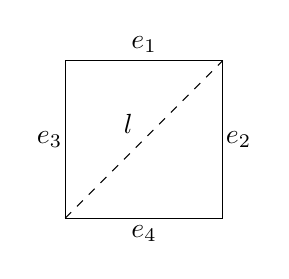
\begin{tikzpicture}
			\def \l{2};
			\def \d{0.2};
			\def \del{0};
			\draw[] (0, 0) rectangle (\l, \l);
			\draw[dashed] (-\del, -\del) -- (\l+\del, \l+\del);
			\node[] at (\l/2, \l+\d) {$e_1$};
			\node[] at (\l+\d, \l/2) {$e_2$};
			\node[] at (-\d, \l/2) {$e_3$};
			\node[] at (\l/2, -\d) {$e_4$};
			\node[] at (\l/2-\d, \l/2+\d) {$l$};
		\end{tikzpicture}
	\end{center}
Then, $G = \langle x, y | x^4 = y^2 = 1, yx = x^3y\rangle.$\\
Where $x \longrightarrow$ rotation by $2\pi/4$ about center and $y \longrightarrow$ reflection about line $l.$\\
$|D_4| = 8.$\\
Let $X = \{e_1, e_2, e_3, e_4\} \longleftarrow$ edges of the square.\\
$G$ acts on $X$ in the natural way.\\
$O_{e_1} = X.$ $G_{e_1} = \{1, xy\}.$
\end{enumerate}
Suppose $g_1, g_2 \in G$ and $x \in X$ such that $g_1x = g_2x.$\\
Observe that $g_1x = g_2x \iff g_2^{-1}(g_1x) = x \iff (g_2^{-1}g_1)x = x \iff g_2^{-1}g_1 \in G_x.$\\
That is equivalent to saying $g_1 \in g_2G_x.$\\~\\
Suppose $y = gx$ is given and we have $G_x.$ Can we find $G_y?$\\
$G_y = \{g_1 \in G : g_1 y = y\} = \{g_1 \in G : g_1(gx) = gx\} = \{g_1 \in G : g^{-1}g_1gx = x\}$\\
$\iff G_y = \{g_1 \in G : g^{-1}g_1g \in G_x\} = \{g_1 \in G : g \in gG_xg^{-1}\}.$\\
$\iff G_y = gG_xg^{-1}.$\\
Thus, if we know the stabiliser of $x,$ we can find the stabiliser of any element in the orbit of $x.$

\subsection{Action on cosets}

$G \longleftarrow$ group and $H \le G.$ $G/H \longleftarrow $ set of all cosets of $H$. ($H$ is not necessarily normal, so $G/H$ is not necessarily a group.)\\
There is a natural action of $G$ on $G/H:$
\[G \times G/H \to G/H\]
\[(g, C) \mapsto gC\]
We take $H \in G/H,$ then we get that $O_H = G/H.$ Thus, this action is transitive.\\
Also, $G_H = H.$ Thus, by our previous result, we get that $G_{aH} = aHa^{-1}.$\\~\\
\textbf{Example}\\
Let $G = S_3$ and $H = \langle  (12)\rangle.$ That is, $H = \{1, (12)\}.$\\
Then, $G/H = \{H, (13)H, (23)H\} = \{a_1, a_2, a_3\}$ where $a_1 = \{1, (12)\}, \; a_2 = \{(13), (123)\}$ and $a_3 = \{(23), (132)\}.$\\
Let $s = (13)H.$ Then, $O_s = G/H.$ (We had noted the action is transitive before as well.)\\
$G_s = (13)H(13)^{-1} = \{1, (23)\}.$\\
Let us observe one more thing:\\
For a fixed $g \in S_3,$ define $m_g : G/H \to G/H$ as left multiplication by $g.$\\
Let $g = (12).$ Under this map, we see the following
\begin{align*}
	a_1 & \mapsto a_1\\
	a_2 & \mapsto a_3\\
	a_3 & \mapsto a_2
\end{align*}
With a slight abuse of notation, we can write it as $m_{(12)} = (a_3, a_2).$
Similarly, we get that $m_{(13)} = (a_2, a_1)$ and $m_{(123)} = (a_1, a_2, a_3).$\\
What we have observed is that there is a natural correspondence from the elements of $G$ to $S_3.$

\hrulefill

In general, given an action $G \times S \to S,$ we get a map $m : G \to \operatorname{Perm}(S)$ defined as $g \mapsto m_g.$\\
If we take two elements of the group - $g_1$ and $g_2,$ we see that $m(g_1g_2) = m_{g_1g_2}.$\\
Note that $m_{g_1g_2}$ is a function from $S$ to $S.$ Given any element $x \in S,$ we get that $m_{g_1g_2}(x) = (g_1g_2)x.$ By our axioms of group action, we get that it is equal to $g_1(g_2 x) = m_{g_1}(m_{g_2}(x)).$\\
This shows that $m_{g_1g_2} = m_{g_1}\circ m_{g_2}.$ Recall that the set of permutations (self bijections) of a set form a group under composition. Thus, what we have shown is that the above map $m$ is in fact a group homomorphism from $G$ to $\operatorname{Perm}(S).$\\~\\
Moreover, $\ker m = \{g \in G : m_g = \operatorname{id}_S\} = \{g \in G : m_g(s) = s \quad \forall s \in S\} = \{g \in G : gs = s \quad \forall s \in S\}.$\\
$\iff \ker m = \displaystyle\bigcap_{s \in S}G_s.$\\
This also shows that the intersection of all the stabilisers is a normal subgroup. Moreover, if it is non-trivial, we get a non-trivial normal subgroup of $G.$

\section{Orbit - Stabiliser Theorem}

Let $G$ be a group acting on a set $X.$ Take $x \in X.$ Consider the following natural map
\[G \overset{\phi}{\longrightarrow}O_x \text{ defined as }g \overset{\phi}{\mapsto}gx.\]
This is a surjective map. Let $g_1 \in gG_x.$ Then $g_1 = gg'$ for some $g' \in G_x.$\\
Then, $g_1 \overset{\phi}{\mapsto}g_1x = (gg')x = g(g'x) = gx = \phi(g).$\\
Thus, every element in the same coset of $G_x$ goes to the same element.\\
This gives us a natural isomorphism defined in the following manner:
\[G/G_x \overset{\psi}{\longrightarrow}O_x \text{ defined as }gG_x \mapsto gx.\]
This map is well defined due to our observations earlier. It is easy to show that this is one-one and onto.\\
This gives us that $|O_x| = [G:G_x].$
\begin{cor}
	When $G$ is a finite set acting on $X,$ we have that
	\[|G| = |G_x||O_x|.\]
\end{cor}
Recall that if $G$ acts on $X,$ then $m_g : X \to X$ was a bijection for all $g$ and we got a group homomorphism $m : G \to \operatorname{Perm}(X)$ by sending $g$ to $m_g.$ \\
We had derived that $\ker m = \displaystyle\bigcap_{x \in X}G_x.$\\
If it is the case that $\ker m = (1),$ then $G$ can be thought of as a subgroup of $\operatorname{Perm}(X)$ as $m:G \to m(G)$ is an isomorphism and $m(G) \subset X.$

\section{Simple groups}
\begin{defn}
	A group $G$ is simple if it has no nontrivial normal subgroups.
\end{defn}
In the above, trivial subgroups mean - $(1)$ and $G.$\\
\textbf{Example:}\\
Let $G$ be a finite group of order $n.$ Let $H \lneq G$ such that $[G:H] = r.$ $G$ acts on $G/H$ by left multiplication.\\
\[m : G \longrightarrow \operatorname{Perm}(G/H) \cong S_r\]
If $n \nmid r!,$ then $m$ is not one-one. (One-one would mean that $m(G)$ has order $n$ but $m(G) \le \operatorname{Perm}(G/H).$)\\
Thus, the kernel is not $(1).$\\
$\ker m = \displaystyle\bigcap_{a \in G}G_{aH} = \displaystyle\bigcap_{a \in G}aHa^{-1} \le H \lneq G.$\\
Thus, $\ker m$ is not equal to the whole group either. This gives us that $\ker m$ is a nontrivial normal subgroup. Thus, $G$ is not simple.\\~\\
The above example also shows that given $H\le G,$ we know that $\displaystyle\bigcap_{g\in G}gHg^{-1} \trianglelefteq G.$\\
Also, $\displaystyle\bigcap_{g \in G}ghg^{-1}$ is the largest normal subgroup of $G$ contained in $H.$

\hrulefill

\textbf{A side note:} Given $G \longleftarrow$ group and $H \le G,$ $H/G$ is the set of right cosets of $H$ in $G.$ If we define an map $G \times H/G \to H/G$ as $(g, C) \mapsto Cg,$ this won't satisfy the axioms of group action in general.\\
Thus, we define $g\cdot C$ as $C\cdot g^{-1}.$

\hrulefill

$G$ acts on $S = \pset (G) \setminus \{\emptyset\}$ with $(g, C) := gC = \{gc : c \in C\}.$\\~\\
We saw that if $G$ acts on $X,$ then $m:G\to\operatorname{Perm}(X)$ is a homomorphism.\\
Conversely, if $\varphi : G \to \operatorname{Perm}(X),$ then we can define $f:G\times X \to X$ as $(g, x) \mapsto (\varphi(g))(x).$ Then, $f$ is a group action.\\
Moreover, the homomorphism corresponding to $f$ turns out to be $\varphi.$ Thus, there is a bijection between these objects.\\
\begin{theorem}[Cayley]
	Let $G$ be a group and $X = G/H$ where $H = (1) \le G.$\\
	Let $\varphi$ be the natural action of $G$ on $X.$\\
	Then, $m : G \to \operatorname{Perm}(X)$ has its kernel given by -\\
	$\ker m = \displaystyle\bigcap_{g \in G}gHg^{-1} = \displaystyle\bigcap_{g \in G}\{1\} = (1).$\\
	Thus, $m$ is injective.\\
	This shows that $G$ can embedded into $\operatorname{Perm}(G).$ That is, it can be seen as a subgroup of a symmetric group.
\end{theorem}
\begin{defn}
	If $m$ is injective, then our action is called faithful.
\end{defn}
In case of a faithful action, $1$ is the only $g$ in $G$ such that $gx = x$ for all $x \in X.$\\
$G$ acts on $G$ by conjugation.\\
$G \times G \to G$ defined as $(g, x) \mapsto gxg^{-1}.$\\
$O_x = \{gxg^{-1} : g \in G\}.$ If a normal subgroup contains $x,$ then it must contain $O_x.$\\~\\
$\varphi_g : G \to G$ given by $x \mapsto gxg^{-1}$ is an automorphism.\\
Moreover, $m : G \to \Aut G$ given by $g \mapsto \varphi_G$ is a homomorphism.\\~\\
Suppose $G$ is generated by $g_1$ and $g_2.$ Let $H \le G.$ If $\varphi_{g_1}(H) = \varphi_{g_2}(H) = H,$ then $\varphi_{g}(H) = H \quad \forall g \in G.$\\
This will follow from the fact that $g \mapsto \varphi_g$ is a homomorphism.\\
Given $x \in G,$ we get that $O_x = [x] \longleftarrow$ conjugacy class of $x$ in $G.$\\
Moreover, the stabiliser $G_x = \{g \in G : xg = gx\}.$ This called the centraliser of $x.$\\
Also, we have the homomorphism $m : G \to \Aut G$ whose kernel is given by $\ker m = \displaystyle\bigcap_{x \in G}G_x = Z(G) \longleftarrow$ center of $G.$\\~\\
%\\
$x \in Z(G) \iff Z(x) = G \iff O_x = C(x) = \{x\}.$\\
In general, $x \notin Z(G) \implies Z(G) \subsetneq Z(x)$ and $x \in Z(G) \implies Z(x) = G.$

\section{Class Equation}

$G$ is the disjoint union of orbits, that is, conjugacy classes.\\
In general, $G = \displaystyle\bigsqcup_{x \in S \subset G}C(x)$ which gives us that $|G| = \displaystyle\sum_{x\in S\subset G}|C(x)|.$\\
The above is known as the class equation.\\
($S$ is a subset of $G$ with the property that given any $x\in G,$ there is exactly one member $|S\cap C(x)| = 1.$)\\
Observation: Given a finite group $G$ such that $|G| = 1 + 1 + \cdots + 1 + n_1 + \cdots + n_k$ is the class equation, (where $n_i > 1$ for all valid $i$) we know the following: The number of $1$s, say $n,$ is the cardinality of $Z(G).$ Moreover, given any $n_i,$ $n < |G|/n_i < |G|$ and $n \mid |G|/n_i \mid |G|.$ (Each $n_i$ actually represents the cardinality of the \emph{orbit} of some element in $G.$)\\
\textbf{Examples.}
\begin{enumerate} 
	\item Find the class equation of $G = S_3.$\\
	$Z(G) = \{1\}.$ Also, $O_x = \{x, x^2\}.$ That is, $|O(x)| = 2.$\\
	The only possibility left for $|O_y|$ is $3.$\\
	Thus, the class equation is $|G| = 1 + 2 + 3.$
	\item Find the class equation of $G = D_4.$\\
	$Z(D_4) = \{1, x^2\}.$\\
	Thus, $|G| = 1 + 1 + \text{something}.$\\
	For $x \in G\setminus Z(G),$ we have it that $Z(G) \lneq Z(x) \lneq G.$ As $|Z(G)| = 2$ and $|G| = 8,$ the only possibility is $|Z(x)| = 4$ or $|O(x)| = 2.$ This gives us that the ``something" can only consist of $2$s. As we have $6$ left, we get that $|G| = 1 + 1 + 2 + 2 + 2.$
	\item Let $G$ be a group such that $|G| = 10.$ Show that $1 + 1 + 1 + 2 + 5$ cannot be the class equation.\\
	$Z(G)$ cannot have 3 elements. \hfill $\blacksquare$
	\item Show that $1 + 1 + 2 + 2 + 2 + 2$ is not possible.\\
	We are given that $|Z(G)| = 2$ and $|Z(x)| = 10/2 = 5$ for some $x \in G.$ But this is a contradiction as $|Z(G)|$ should divide $|Z(x)|$ but $2 \nmid 5.$
\end{enumerate}

\begin{defn}
	If $|G| = p^n$ for some prime $p$ and $n \in \mathbb{N},$ then $G$ is said to be a $p-$group.
\end{defn}
\begin{theorem}
	If $G$ is a $p-$group, then $Z(G) \neq (1).$
\end{theorem}
\begin{proof}
	Assume $Z(G) = 1,$ then the class equation will give us that:
	\[p^n = 1 + p^{\alpha_1} + \cdots p^{\alpha_k}.\]
	This is a contradiction as the left hand side is divisible by $p$ but the right hand side is not.
\end{proof}
\begin{theorem}
	If $|G| = p^2$ for some prime $p,$ then $G$ is abelian.
\end{theorem}
\begin{proof}
	By the previous theorem, we know that $|Z(G)| > 1.$ If $|Z(G)| = p^2,$ then we are done. Assume not. Then, $|Z(G)| = p.$\\
	Thus, $G \setminus Z(G)$ is nonempty. Let $x \in G\setminus Z(G).$ Then, we have it that $Z(G) \lneq Z(x) \lneq G.$ However, considering the divisibilities of orders, this is not possible.
\end{proof}
\begin{theorem}
	If $|G| = p^2$ for some prime $p,$ then $G \cong \mathbb{Z}/p^2\mathbb{Z}$ or $G \cong (\mathbb{Z}/p\mathbb{Z})\times (\mathbb{Z}/p\mathbb{Z}).$
\end{theorem}
\begin{proof}
	$G$ contains an element of order $p^2,$ then $G$ is cyclic and we are done.\\
	Assume $G$ does not have an element of order $p^2.$ In that case, all elements $(\neq1)$ have order $p.$\\
	Choose $1 \neq x \in G.$ Choose $y \in G \setminus \langle x\rangle.$\\
	Then, we have it that $\langle x\rangle \cong \langle y\rangle \cong \mathbb{Z}/p\mathbb{Z}.$ Moreover, $\langle x\rangle \cap \langle y\rangle = (1).$\\
	As $G$ is abelian, by previous theorem, we also have it that $\langle x\rangle \langle y\rangle = \langle y\rangle\langle x\rangle .$\\
	Lastly, we also have it that $\langle x\rangle\langle y\rangle = G.$ Thus, $G \cong \langle x\rangle\times\langle y\rangle$ and we are done.
\end{proof}

\section{Classification Theorems}
\begin{theorem}[Classification of finite Abelian Groups]
	Let $G$ be a finite abelian group.\\
	$|G| = p_1^{n_1}\cdots p_k^{n_k} : p_i$s are distinct primes.\\
	Then, $G \cong G_1 \times G_2 \times \cdots \times G_k$ where $|G_i| = p_i^{n_i}$ for each valid $i.$\\
	Now, let us assume that $|G| = p^n.$\\
	For each partition $\mathcal{P}$ of $n$ such that $\mathcal{P} = (t_1, t_2, \ldots, t_s)$ and $\displaystyle\sum_{k=1}^{s}t_k = n,$ define the following:
	\[G_{\mathcal{P}} := (\mathbb{Z}/p^{t_1}\mathbb{Z}) \times \cdots \times \left(\mathbb{Z}/p^{t_s}\mathbb{Z}\right).\]
	Then, $G \cong G_\mathcal{P}$ for some partition $\mathcal{P}.$
\end{theorem}
\begin{theorem}[Classification of finitely generated Abelian Groups]
	Let $G$ be a finitely generated abelian group.\\
	Then, $G \cong \mathbb{Z}^r \times T$ for some natural number $r$ and group $T$ such that $|T| < \infty.$ This $r$ is known as the rank of $G.$
\end{theorem}

\section{Conjugation in \texorpdfstring{$S_n$}{Sn}}
Let $p \in S_n$ and $q \in S_n.$ We can visualise $qpq^{-1}$ easily in terms of $q$ by replacing each element $i$ in the cycle representation of $p$ with $q(i).$\\
Example: Let $p = (123)(457)$ and $q = (134267).$ Then $qpq^{-1} = (q(1), q(2), q(3))(q(4), q(5), q(7)) = (364)(251).$\\
Thus, all conjugates of an element have the same cycle type. Moreover, it can be easily seen that given any element $y$ of the same cycle type as $x,$ one can find a $q \in S_n$ such that $y = qxq^{-1}.$\\
Thus, the conjugacy class of any element $p$ consists of all the elements of the same cycle type as $p.$\\
\begin{theorem}
	Two permutations $p, q \in S_n$ are conjugates iff $p$ and $q$ have the same cycle type.
\end{theorem}
Thus, one can now find the class equations of $S_n$ (relatively) easily.\\
\textbf{Example:} Find the class equation of $S_4.$\\
Let us consider the possible cycle types and the number of elements with that cycle type:\\
$id \longrightarrow $1\\
$(12) \longrightarrow \frac{1}{2}^4P_2 = 6$\\
$(123) \longrightarrow \frac{1}{3}^4P_3 = 8$\\
$(1234) \longrightarrow \frac{1}{4}^4P_4 = 6$\\
$(12)(34) \longrightarrow \frac{1}{2!}\left(\frac{1}{2}^4P_2\right)\left(\frac{1}{2}^2P_2\right) = 3$\\
Thus, the class equation is $|S_4| = 1 + 6 + 8 + 6 + 3.$

Facts:
\begin{enumerate}[nosep] 
	\item $S_n$ is generated by transposition.
	\item $A_n$ is generated by $3-$cycles.
	\item If $ n \ge 5,$ then all $3-$cycles are conjugates in $A_n.$
\end{enumerate}

\begin{theorem}
	If $n \ge 5,$ then $A_n$ is simple. That is, $A_n$ has no nontrivial normal subgroups.
\end{theorem}
\begin{proof}
	Let $(1) \neq H \trianglelefteq A_n.$ \\
	We shall prove the theorem by showing that $H$ contains a $3-$cycles. As $H$ is normal, it must contain all the conjugates (in $A_n$) of this $3-$cycle. By the last fact above, this would then contain all the $3-$cycles. By the second fact, we'll get that $A_n \subset H$ and thus, proving that $H = A_n.$\\
	Rest is omitted.
\end{proof}
$G$ acts on $ S = \pset (G) \setminus \{\emptyset\}$ by conjugation.\\
$\varphi : G\times S \to S$ such that $(g, A) \overset{\varphi}{\mapsto}gAg^{-1}.$\\
Let $H' \le G.$ $O_H = $ all conjugate subgroups of $H.$\\
$G_H = \{g \in G:gHg^{-1} = H\} = N_G(H)  \longleftarrow$ normaliser of $H$ in $G.$\\
$H \trianglelefteq N_G(H) \longleftarrow$ largest subgroup of $G$ containing $H$ such that $H$ is normal in that.\\
$|G| = |O_H||G_H|.$ Thus, $[G:G_H] = |O_H|.$\\
$H\trianglelefteq G$ iff $N_G(H) = G$ iff $O_H = \{H\}.$\\~\\
%\\
\textbf{Example:}\\
$x = (12)(34) \in G = S_5.$ $H = \langle x\rangle.$\\
What is $N_G(H)?$\\
It is clear that $|H| = 2.$ Also, $O_H$ (under conjugation) consists of all the elements of $S_5$ which have cycle type $2, 2, 1.$ There are $15$ such elements. Thus, $|N_G(H)| = |G_H| = |G|/|O_H| = 8.$\\
Also, note that if $g = g_1g_2\cdots g_r \longleftarrow$ product of disjoint cycles, then each $g_i \in Z(g) = N_G(\langle g\rangle)$ as each $g_i$ will commute with $g.$\\
Thus, we already have it that $(12)$ and $(34)$ belong to $N_G(H).$ Thus, $\langle (12), (34)\rangle \subset N_G(H).$ We still need $4$ more elements.\\
Note that if we find the element that conjugates $(12)$ to $(34),$ even that must belong to $N_G(H).$ That element can be easily found to be $(13)(24).$\\
Thus, $N_G(H) = \langle (12), (34), (13)(24)\rangle \longleftarrow$ check that this contains $8$ elements.

\section{Conjugation in \texorpdfstring{$A_n$}{An}}

Given $p \in S_n,$ we know that all of its conjugates in $S_n$ are precisely those permutations that have the same cycle type. However, they may not be conjugates in $A_n.$ \\
Let $p \in S_n.$ We know that $|C_{S_n}(p)| = \dfrac{|S_n|}{|Z_{S_n}(p)|}.$\\
Similarly, $|C_{A_n}(p)| = \dfrac{|A_n|}{|Z_{A_n}(p)|}.$\\~\\
Case 1. Suppose it is the case that $Z_{S_n}(p)$ does not contain any odd permutation. This means that $|Z_{S_n}(p)| = |Z_{A_n}(p)|$ and thus, $|C_{A_n}(p)| = \dfrac{|A_n|}{|Z_{A_n}(p)|} = \dfrac{\frac{1}{2}|S_n|}{|Z_{S_n}(p)|} = \dfrac{1}{2}|C_{S_n}(p)|.$\\
Case 2. Suppose it is the case that $Z_{S_n}(p)$ does contains an odd permutation. Let $\sigma$ be any such permutation. Let $H = Z_{S_n}(p) \cap A_n.$ That is, the set of all even permutations in $Z_{S_n}(p).$ Moreover, this is a subgroup.\\
Let $\tau$ be an odd permutation in $Z_{S_n}(p).$ Note that $Z_{S_n}(p)$ is a subgroup. Thus, $\sigma^{-1}\tau\in Z_{S_n}(p).$ Also, note $\sigma^{-1}\tau$ is an even permutation. Thus, $\sigma^{-1}\tau\in H.$ Or equivalently, $\tau \in \sigma H.$ Thus, we have shown that whenever $\tau$ is an odd permutation in $Z_{S_n}(p),$ it must belong to $\sigma H.$ This shows that $|H| = |Z_{A_n}(p)| = \frac{1}{2}|Z_{S_n}(p)|.$\\
Thus, we get that $|C_{A_n}(p)| = |C_{S_n}(p)|.$\\~\\

\textbf{Example:}\\
Let $G = A_5.$ Take $x = (12345) \in A_5.$\\
We know that number of $5-$cycles in $A_5$ is $24.$ All of these are conjugates in $S_5.$ Are they still conjugates in $A_5?$\\
Let us assume that this is indeed the case. This tell us that $|O_x| = 24.$ However, $24$ does not divide $|A_5| = 60.$ Thus, it cannot be the case.\\
We have shown above that the only other possibility is for $|O_x|$ to be $24/2 = 12.$\\
What this means is that there are two conjugacy classes in $A_5$ that consist of $5-$cycles.

\section{Sylow Theorem}
$G \longleftarrow $ group. \\
$|G| = p^\alpha m$ where $\alpha \ge 1,$ $p \to$ prime, $p \nmid m.$\\
$\Syl_p(G) = \{\text{subgroups of }G\text{ of order }p^\alpha\}.$\\
An element of $\Syl_p(G)$ is called a Sylow $p-$subgroup of $G.$\\
$n_p(G) := |\Syl_p(G)|.$

\begin{theorem}[Sylow]
	There are three parts to the theorem:\\
	\textbf{First.} $n_p \ge 1.$\\
	\textbf{Second.}
	\begin{enumerate}[nosep] 
		\item All Sylow $p$ subgroups of $G$ are conjugates.
		\item If $H$ is a $p-$group, then $H$ is contained in some Sylow $p-$subgroup.
	\end{enumerate}
	\textbf{Third.}
	\begin{enumerate}[nosep] 
		\item Fix $M \in \Syl_p(G).$\\
		$n_p = |O_M| \longleftarrow$ number of conjugacy classes of $M$\\
		$[G:N_G(M)] = n_p$\\
		$\implies |N_G(M)| = \frac{|G|}{n_p} = \frac{p^\alpha m}{n_p}.$\\
		Also, $M \le N_G(M).$ As $|M| = p^\alpha,$ we get that $p^\alpha \mid |N_G(M)|.$
		\begin{enumerate}[nosep] 
			\item $n_p \mid m$
			\item $n_p \equiv 1 \mod p$
		\end{enumerate}
	\end{enumerate}
\end{theorem}
\textbf{Consequences:} Let $G$ be a finite group.
\begin{enumerate} 
	\item If $p \mid |G|,$ then $G$ has an element of order $p.$
	\begin{proof}
		$|G| = p^\alpha m,$ where $\alpha \ge 1.$
		By Sylow Theorem, there exists $H \le G$ such that $|H| = p^\alpha.$\\
		Choose $1 \neq x \in H.$ Then $\ord(x) = p^\beta$ for some $1 \le \beta \le \alpha.$\\
		Choose $y = x^{p^{\beta - 1}}.$ Then $\ord(y) = p.$
	\end{proof}
	\item If $p \mid |G|$ and $H \in \Syl_p(G),$ then $H \trianglelefteq G$ iff $n_p = 1.$
	\item Assume $|G| = pq$ where $p < q \longleftarrow$ primes.\\
	\begin{proof}
	Then $n_q \mid p.$ Thus, $n_q = 1$ or $p.$\\
	Also, $n_q = 1 + kp$ for some $k \in \mathbb{Z}.$ As $p < q,$ we have it that $n_q = 1.$\\
	Thus, $H \in \Syl_q(G)$ is a nontrivial normal subgroup of $G.$ Thus, $G$ is not simple.
	\end{proof}
	
	\item If $\ord(G) = p,$ then $G$ is abelian and simple. (There are no nontrivial subgroups to begin with.)
	\item If $\ord(G) \neq$ prime and $G$ is abelian, then $G$ is not simple.
	\begin{proof}
	Using (1), we get that $G$ has a proper subgroup. As $G$ is abelian, this is normal.
	\end{proof}
	\item If $|G| = p^\alpha$ for prime $p$ and $\alpha \ge 2,$ then $G$ is not simple.
	\begin{proof}
		As $G$ is a $p-$group, $Z(p) \neq (1).$\\
		If $Z(G) = G,$ then $G$ is abelian and we are done by (5).\\
		If $Z(G) \neq G,$ then we have it that $Z(G)$ is a nontrivial normal subgroup of $G$ and we are done.
	\end{proof}	
	\item $|G| = p^2q.$ $p, q \longleftarrow$ primes, then $G$ is not simple.
	\begin{proof}
		(i) $p > q.$ Then similar arguments as (3) show that $n_p = 1$ and thus, we are done.
		(ii) $p < q.$ Then $n_q \mid p^2$ and $n_q \equiv 1 \mod q.$ If $n_q = 1,$ then we are done. Assume $n_q \neq 1.$ If $n_q = p,$ then $p = 1 + kp$ for some $k \in \mathbb{N}.$ This is not possible as $q > p.$\\
		Thus, the only possibility left is that $n_q = p^2.$\\
		In that case, $\Syl_q(G) = \{P_1,\;P_2, \ldots,\; P_{p^2}\}$ such that $P_i$ has prime order ($q$) for all valid $i.$\\
		Given $i \neq j,$ $P_i$ and $P_j$ are distinct. Thus, $P_i \cap P_j$ is a proper subgroup of $P_i.$ As $P_i$ has prime order, we have it that $P_i \cap P_j = (1).$\\
		Thus, if we calculate the number of elements in $G$ that have order $q,$ we get that it is:\\
		$n = p^2(q - 1).$\\
		Thus, the number of element remaining is $p^2q - p^2(q^2 - 1) = p^2.$\\
		By Sylow Theorem, these remaining $p^2$ elements \emph{have} to form a subgroup. More importantly, this is the only subgroup of order $p^2.$ \\
		Thus, $n_p = 1.$ $\implies G$ is not simple.
	\end{proof}
	\item $|G| = pqr.$ $p < q < r \longleftarrow$ primes.\\
	For sake of contradiction, assume that $n_r, n_q, n_p > 1.$\\
	By arguments similar to previous ones, we know that $n_r$ must be $pq.$\\
	$\#$ of elements of order $r = pq(r-1).$\\
	$n_q > 1, \; n_q \equiv 1 \mod q$ and $n_q \mid pr$ gives us that $n_q \ge r.$ 
	$\therefore \#$ of elements of order $q \ge r(q-1).$\\
	Similarly, we get that $n_p \ge q$ and hence, $\#$ of elements of order $p \ge q(p-1).$\\
	The above number are counting distinct elements. Thus, we get that -\\
	$|G| \ge pq(r-1) + r(q-1) + q(p-1) = pqr + (r-1)(q-1) > pqr.$ A contradiction. 
\end{enumerate}
\begin{theorem}
	Suppose $|G| \le 200$ and $60 \neq |G| \neq 168$ and $|G|$ is not a prime. Then, $G$ is not simple.
\end{theorem}
\end{document}